\chapter{XỬ LÝ NGẮT}
\section{Giới thiệu chung}
\subsection{Yêu cầu}
Viết chương trình xử lý ngắt với nút nhấn.
\subsection{Hoạt động ngắt}
Ngắt là một tín hiệu điều khiển bắt vi điều khiển tạm ngưng công việc đang thực hiện để tiến hành các thao tác khác do ngắt quy đinh qua chương trình ngắt.

Khi phát hiện ngắt thì vi điều khiển sẽ thực hiện một chương trình độc lập với chương trình chính gọi là chương trình ngắt.\\

Cấu trúc của một chương trình ngắt:
\begin{itemize}
\item Bắt đầu là tên ngắt: \verb|#INT_tên_ngắt| với \verb|tên_ngắt| ta có thể xem trong chương trình CCS (trong \verb|View/Valid Interrupts|).
\item Kế tiếp là \emph{chương trình ngắt} (tùy theo mục đích mà chúng ta viết chương trình hoạt động khi xảy ra ngắt).
\begin{verbatim}
tên_hàm(){
    //Nội dung chương trình ngắt
}
\end{verbatim}
\end{itemize}
\section{Thiết lập hoạt động ngắt}\label{Sec:int}
Sử dụng các lệnh sau để thiết lặp hoạt động ngắt:
\begin{itemize}
\item \verb|ENABLE_INTERRUPTS(level);| với \verb|level| là \verb|INT_tên_ngắt| hoặc \verb|GLOBAL| (ngắt toàn cục): cho phép ngắt.
\item \verb|DISABLE_INTERRUPTS(level);| với \verb|level| giống như trên: vô hiệu hóa ngắt.
\item \verb|CLEAR_INTERRUPT(level);| với \verb|level| không có \verb|GLOBAL|: xóa cờ ngắt.
\item \verb|EXT_INT_EDGE(soure, edge);| với:
\begin{itemize}
\item \verb|soure = 0, 1, 2|: nguồn ngắt (ứng với \verb|EXT0|, \verb|EXT1|, \verb|EXT2|).
\item \verb|edge = L_TO_H, H_TO_L|: cạch kích ngắt (mức thấp lên cao hoặc mức cao xuống thấp).
\end{itemize}
\end{itemize}

Thiết kế chương trình có dùng ngắt:
\begin{itemize}
\item Trong hàm \verb|main()|: cho phép ngắt cụ thể (\verb|tên_ngắt|), ngắt toàn cục (\verb|GLOBAL|) và đợi ngắt (\verb|EXT_INT_EDGE|).
\item Chương trình xử lý ngắt (đặt trước hàm \verb|main()|): xóa cờ ngắt (\verb|CLEAR_INTERRUPT|), cấm ngắt toàn cục (\verb|DISABLE_INTERRUPTS(GLOBAL);|) xử lý chương trình ngắt xong rồi cho phép ngắt toàn cục lại (\verb|ENABLE_INTERRUPTS(GLOBAL);|)
\end{itemize}
\section{Bài tập}
\subsection{Bài tập 3.1}
\paragraph{Yêu cầu}Viết chương trình nhận nút nhấn ở chân B0 của PIC 16F887, cứ mỗi lần nhấn phím sẽ đảo trạng thái các LED ở PORT E.
\paragraph{Hướng giải quyết}
\begin{itemize}
\item Chân \verb|B0| cho phép ngắt ngoài, nên chúng ta sử dụng \verb|#INT_EXT|.
\item Chương trình ngắt: thiết kế như hướng dẫn ở \emph{mục \ref{Sec:int}}, nội dung ngắt là đảo trạng thái PORT E: \verb|PORTE =| $\sim$\verb|PORTE;|
\item Chương trình chính: 
\begin{itemize}
\item Khai báo \verb|PORT B| là chân \verb|INPUT| (nút nhấn): \verb|TRISB = 0xFF;| còn \verb|PORT E| là chân \verb|OUTPUT| (led): \verb|TRISE = 0x00;|
\item Ở \verb|PORT B| khi giao tiếp nút nhấn, cần có điện trở mắc lên nguồn cho chân B0, ta khai báo: \verb|PORT_B_PULLUPS(0x01);|
\item Kích hoạt ngắt ngoài: \verb|ENABLE_INTERRUPTS(INT_EXT);| 
\item Chọn cạnh ngắt: \verb|EXT_INT_EDGE(H_TO_L);| \item Kích hoạt ngắt toàn cục \verb|ENABLE_INTERRUPTS(GLOBAL);|
\item Duy trì hoạt động của vi điều khiển: dùng \verb|while|.
\end{itemize}
%\item[$\ast$] \textit{Lưu ý}: tùy vào phần cứng chúng ta thiết kế có thể sẽ bị nhiễu, dẫn đến xảy ra ngắt khi mới vào chương trình, nếu bị nhiễu thì chúng ta thay đổi trạng thái LED ở PORT E là: \verb|PORTE = 0x00| hoặc \verb|PORTE = 0xFF| để cho phù hợp.
\end{itemize}
\subsection*{Sơ đồ mạch}
\begin{figure}[!h]
\begin{center}
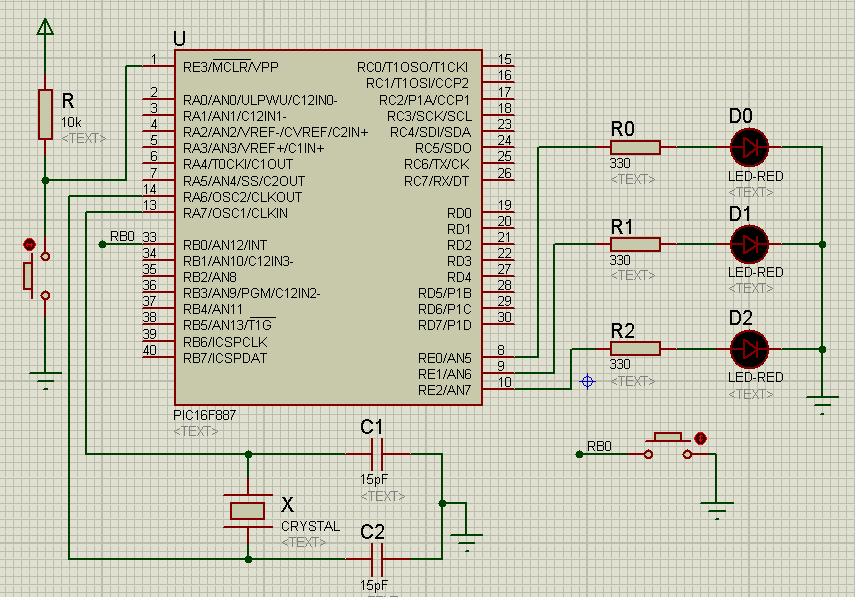
\includegraphics[scale=0.6]{bai-3/image/BAI-3-1}
\end{center}
\caption{Mạch đảo trạng thái LED ở PORT E với ngắt ngoài}
\end{figure}
\subsection*{Chương trình 7}
\lstinputlisting[language=C]{BAI-3-1.C}
\subsection{Bài tập 3.2}\label{Ex:3-2}
\paragraph{Yêu cầu}Viết chương trình hiển thị số lần nhấn phím ở chân B0 của PIC 16F887 lên màn hình LCD 16x02.
\paragraph{Hướng giải quyết}
\begin{itemize}
\item Sử dụng lại \emph{chương trình 7} với một số thay đổi như sau:
\begin{itemize}
\item Khai báo biến \verb|count| là biến toàn cục (để ảnh hưởng đến toàn chương trình).
\item Thay lệnh \verb|PORTE =| $\sim$\verb|PORTE| bằng lệnh \verb|count++|.
\end{itemize}
\item Trong chương trình chính ta thực hiện:
\begin{itemize}
\item Khai báo LCD (được trình bày trong \emph{chương trình 6} của \emph{bài tập 2.3}).
\item Sử dụng vòng lặp \verb|while| để duy trì chương trình: trong vòng lặp cho hiển thị biến \verb|count| lên LCD bằng hàm \verb|printf| kết hợp với hàm \verb|LCD_PutChar|.
\end{itemize}
\item Với các khai báo trên thì chương trình sẽ xảy ra nhiễu (do dội phím, rung do phần cứng), khi đó phải khắc phục nhiễu theo \textit{bài tập 3.4 trang \pageref{Ex:3-4}}.
\item[$\ast$] \textit{Lưu ý}: Khi chúng ta chưa xử lý chống nhiễu thì nó sẽ xảy ra một ngắt không mong muốn.
\item \textit{Hướng giải quyết khác cho bài này}: Ta không dùng ngắt, mà thay vào đó dùng hàm \verb|input(PIN_B0)| để đọc tín hiệu từ nút nhấn. Rồi xử lý chống nhiễu bằng cách thêm hàm \verb|delay_ms(500)| vào lệnh \verb|if| sau khi đọc được nút nhấn.
\item[$\ast$] Trong bài này chúng ta không sử dụng hàm \verb|input| trong \textit{chương trình chính} là do nội dung của bài thực hành là khảo sát ngắt trên vi điều khiển PIC 16F887, nên chọn hàm \verb|input| để sử dụng thì không hợp với nội dung.
\item[$\ast$] Để so sánh chương trình dùng ngắt và chương trình dùng \verb|input|, ta cùng xem chương trình trong \textit{mục \ref{Code:Button 3-2} trang \pageref{Code:Button 3-2}}.
\end{itemize}
\subsection*{Sơ đồ mạch}
\begin{figure}[!h]
\begin{center}
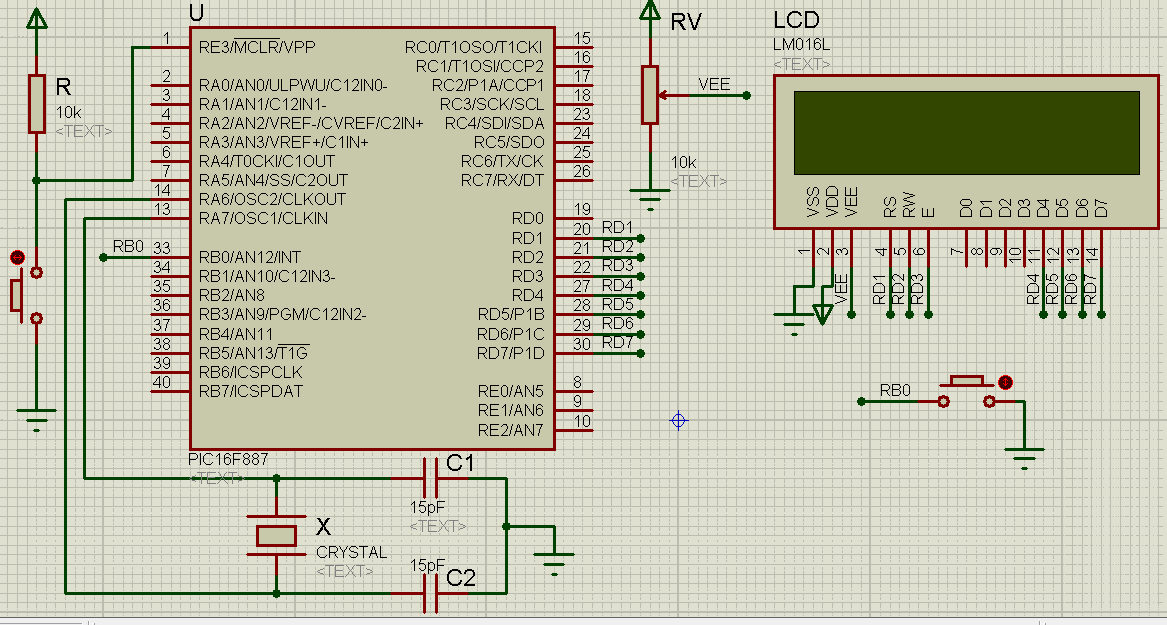
\includegraphics[scale=0.5]{bai-3/image/BAI-3-2}
\end{center}
\caption{Mạch đọc số lần nhấn nút ở chân B0 hiển thị lên LCD}
\end{figure}
\newpage
\subsection*{Chương trình 8}
\lstinputlisting[language=C]{BAI-3-2.C}
\newpage
\subsection{Bài tập 3.3}
\paragraph{Yêu cầu}Viết chương trình nhận nút nhấn ở chân \verb|B3 - B5| của PIC 16F887, hiển thị lên màn hình LCD 16x02.
\paragraph{Hướng giải quyết}
\begin{itemize}
\item Ở PIC 16F877A thì sử dụng các ngắt nối tiếp (từ chân RB4 -- RB7) dễ hơn nhiều so với PIC 16F887.
\item Để đơn giản, chúng ta không sử dụng ngắt nối tiếp mà dùng cách đọc tín hiệu từ các chân B3 -- B5 thông qua hàm input rồi cho xuất ra LCD.
\item Tạo một mảng: \verb|{B3, B4, B5} = {3, 4, 5}|, nếu nhấn nút nhấn ở chân B3 thì xuất ra biến \verb|kt = 3|, tương tự cho các chân còn lại.
\item Kiểm tra giá trị của biến \verb|kt| rồi cho xuất ra LCD thông qua hàm 

\verb|printf(LCD_PutChar)|.
\item Sử dụng điện trở nội cho các chân ở PORT B: \verb|PORT_B_PULL(0x38);| chỉ có 3 chân \verb|B3, B4, B5| được mắc trở lên nguồn.
\item[$\ast$] \textit{Kết luận}: Phần trên là ý tưởng giải quyết bài tập của em, nhưng khi chạy thực tế, vì lý do nào đó mà chân \verb|RB3| không lên mức cao được! Vấn đề này em chưa giải quyết được.
\end{itemize}
\subsection*{Sơ đồ mạch}
\begin{figure}[!h]
\begin{center}
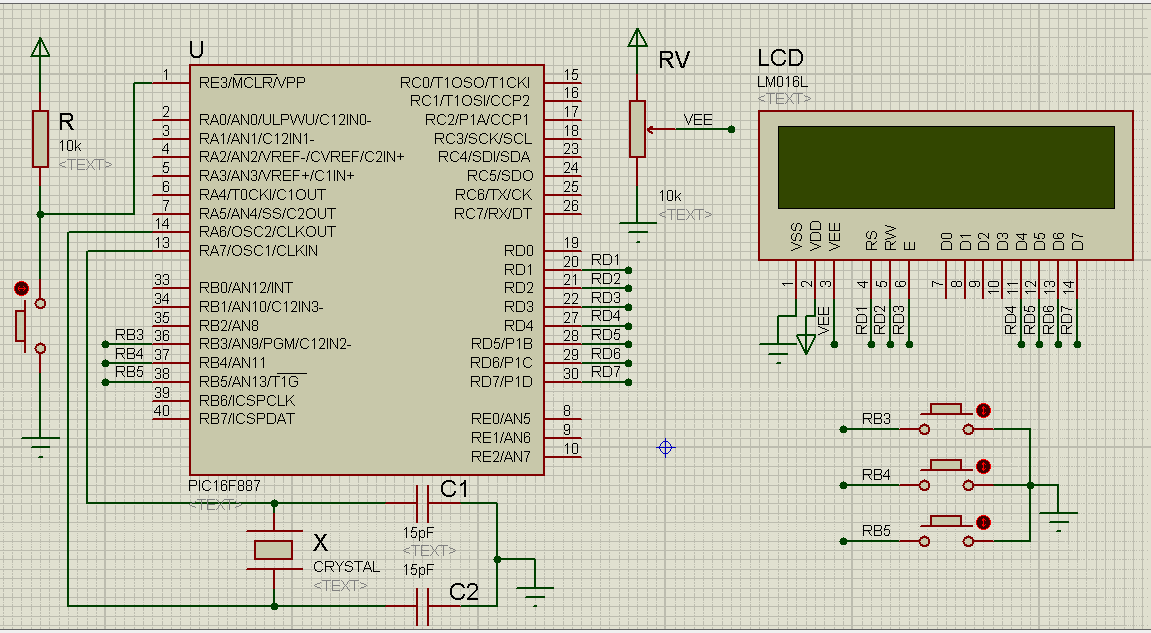
\includegraphics[scale=0.4]{bai-3/image/BAI-3-3}
\end{center}
\caption{Mạch đọc nút nhấn từ chân B3 -- B5 và hiển thị lên LCD}
\end{figure}
%\subsection*{Chương trình 9}
\subsection{Bài tập 3.4}\label{Ex:3-4}
\paragraph{Yêu cầu}Viết chương trình nhận nút nhất ở chân B0 của PIC 16F887 có xử lý chống nhiễu.
\paragraph{Hướng giải quyết}
\begin{itemize}
\item Khi sử dụng nút nhấn, có xảy ra quá trình dội, nhiễu và rung do phần cứng. Cụ thể là ở \emph{bài tập 3.1} khi ta nhấn nút thì LED bị nhiễu. Nên ta cần xử lý chống nhiễu cho tín hiệu.
\item Dùng hàm \verb|delay_ms(số mili giây)| với \verb|số mili giây = 10 - 20ms| để bỏ qua xung nhiễu. Rồi lấy mức 0 làm điều kiện có nút nhấn:

\verb|if input(PIN_B0) == 0| thì thực hiện lệnh cần thiết.
\end{itemize}
\subsection*{Chương trình 9}
\lstinputlisting[language=C]{BAI-3-4.C}
\subsection{Đọc tín hiệu từ nút nhấn với hàm INPUT}\label{Code:Button 3-2}
Nội dung file \verb|INPUT_BUTTON.C| (Một cách làm khác của \textit{bài tập 3.2} trang \pageref{Ex:3-2}).
\subsection*{Chương trình 10}
\lstinputlisting[language=C]{INPUT_BUTTON.C}